\subsection{Exemples de nano ordinateurs qui supportent les \acrshort{sdk} pour l'\acrshort{ia}} \label{annexe:nano_computer_samples}
{
   \renewcommand*{\arraystretch}{1.4}
   \begin{table}[ht]
   \centering
   \caption{Comparaison des trois nano ordinateurs supportant les \acrshort{sdk} pour l'\acrshort{ia}}\label{table:compare_nano}
   \vspace{0.1em} % Adjust the height of the space between caption and tabular
   \begin{tabular}{{@{}|p{12em}|p{12em}|p{12em}|@{}}}
      \hline
      \textbf{NVIDIA Jetson Nano} & \textbf{NVIDIA Jetson Xavier AGX} & \textbf{Raspberry Pi 4B + Intel NCS2}\\
      \hline  
      \centering 99USD & \centering 599USD &  134USD (55USD + 79USD) \\
      \hline
      45 x 69.6 mm, 250 gr, 5-10 W & 100 x 87 mm, 630 gr, 10-15-30 W & 56 x 85.60 mm + 27x72 mm, 45 gr + 18.1 gr, 15 W\\
      \hline
      128-core NVIDIA Maxwell GPU & 512-core NVIDIA Volta GPU with 64 Tensor Cores & Intel Movidius Myriad X VPU 16 SHAVE cores \\
      \hline
      Quad-Core ARM Cortex-A57 MPCore & 8-core NVIDIA Carmel Arm v8.2 64-bit CPU 8MB L2 + 4MB L3 & Quad-core ARM Cortex-A72 64-bit @ 1.5 GHz\\
      \hline
      4 GB 64-bit LPDDR4 & 32 GB 256-bit LPDDR4 & 4GB LPDDR4\\
      \hline
      0.47 TFLOPS@FP16 & 5.5-11.5 TFLOPS@FP16; 20-32 TOPS@INT8 & 4 FLOPS@FP16, 1 TOPS@INT8 \\
      \hline
   \end{tabular}
   \end{table}
}
\subsection{Communication avec l’\acrlong{apcpontjc}}
\noindent L'\acrlong{apcpontjc} (\acrshort{apcpontjc}) a été contacté afin de leur demander la permission d'utiliser leurs fichiers multimédias de la piste cyclable du pont Jacques-Cartier, tel que leurs images et leurs vidéos. Voici les détails de la communication et les conditions d'utilisation.
{
   \centering   
   \label{pdf:courriel_autorisation_apc_pontjc}
   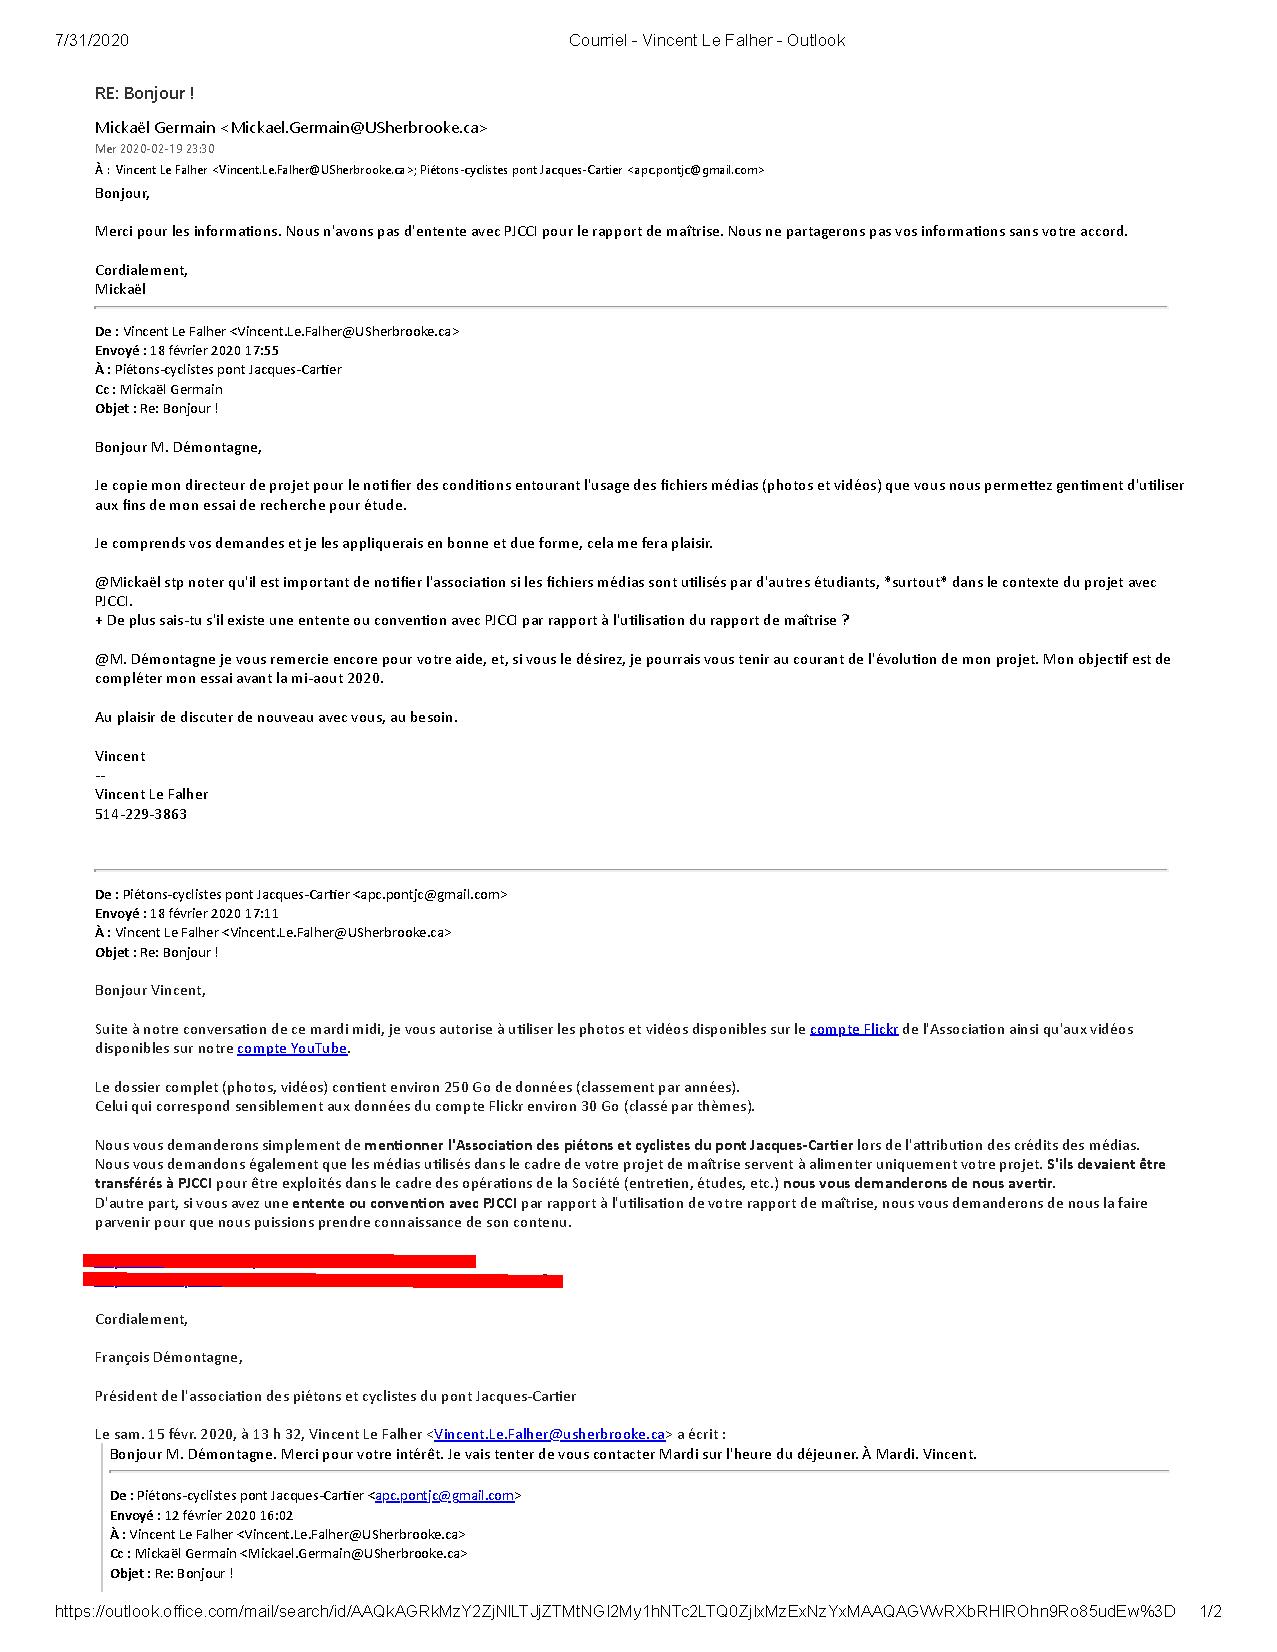
\includegraphics[page=1,width=\textwidth]{courriel_autorisation_apc_pontjc.pdf} \\
   \clearpage
   \includegraphics[page=2,width=\textwidth]{courriel_autorisation_apc_pontjc.pdf} \\
}

% do not used \includepdf, it breaks \printglossary. Prefer using \includegraphics, it works with pdf
% 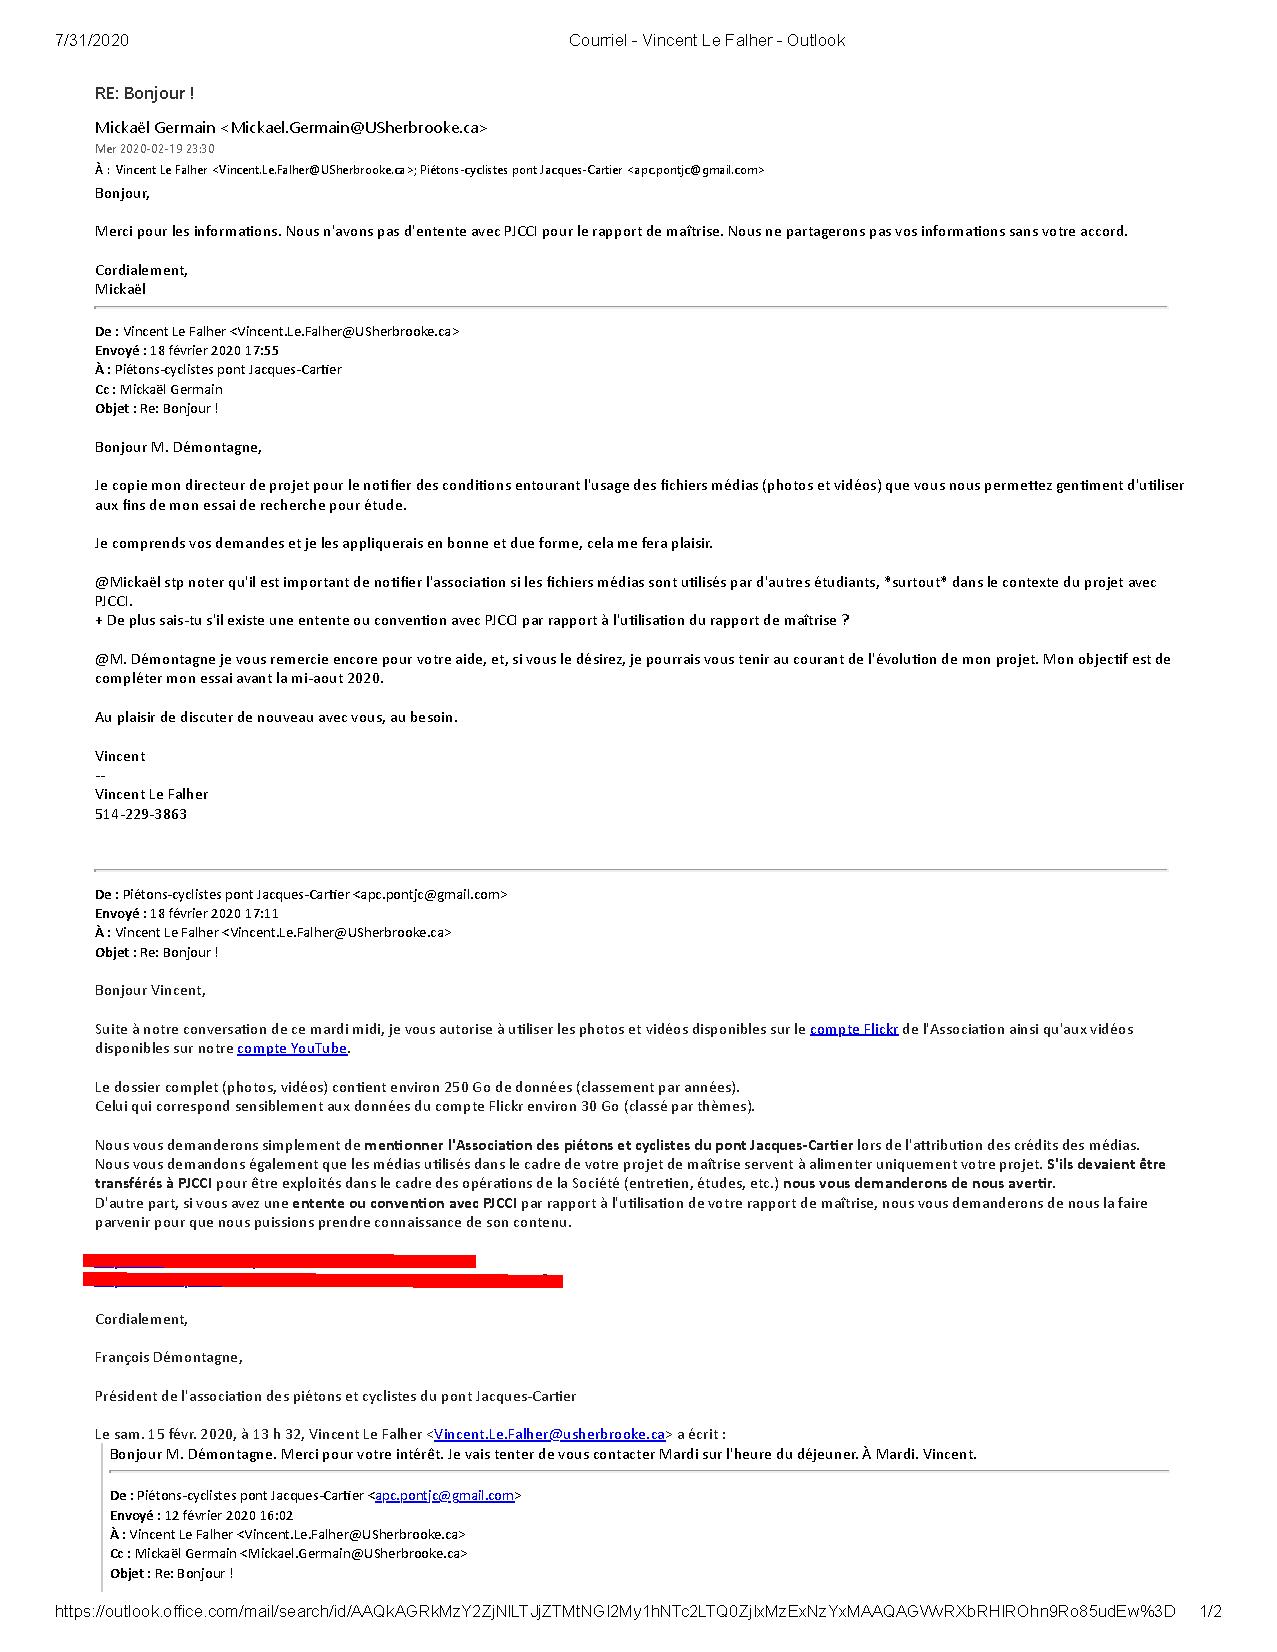
\includepdf[pages=1,width=\textwidth]{courriel_autorisation_apc_pontjc.pdf} \label{pdf:courriel_autorisation_apc_pontjc}
% 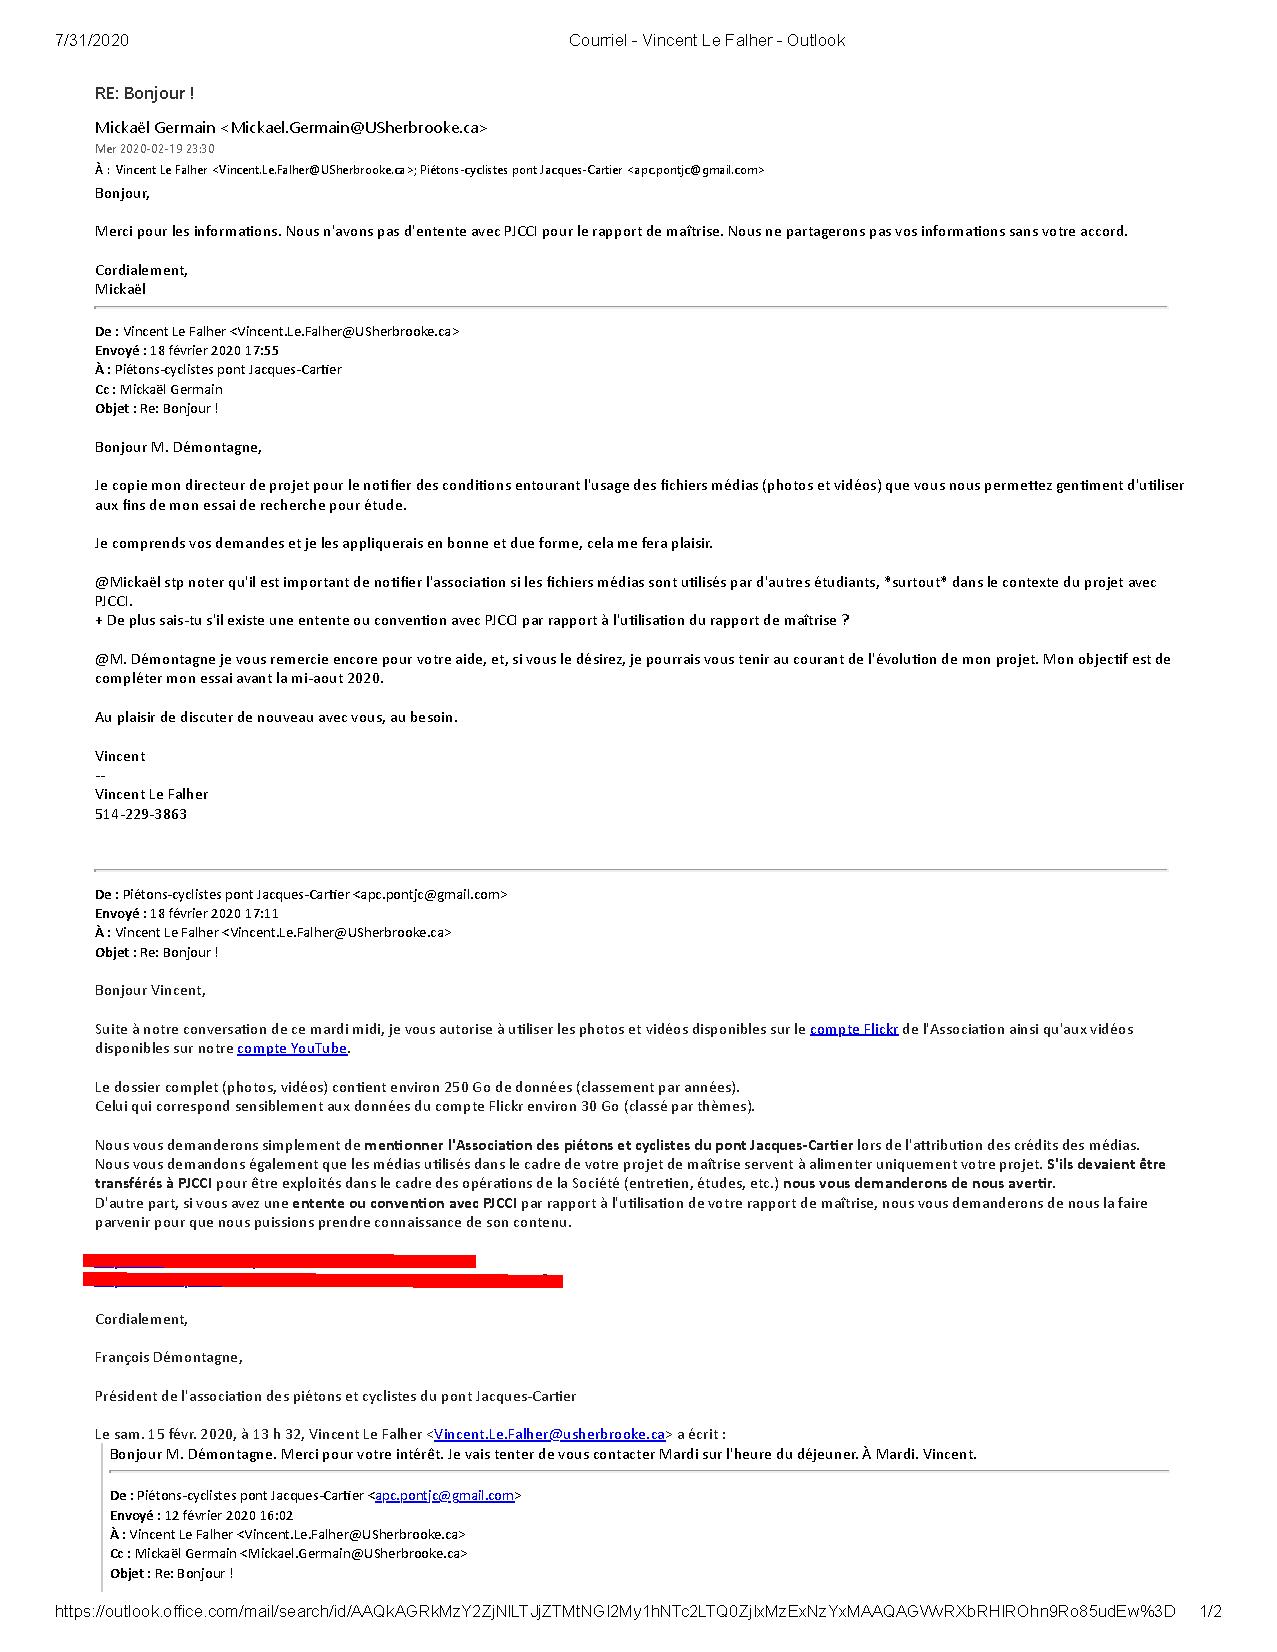
\includepdf[pages=-,pagecommand={},width=\textwidth]{courriel_autorisation_apc_pontjc.pdf} \label{pdf:courriel_autorisation_apc_pontjc}
